\documentclass{article}
\usepackage[margin=0.5in]{geometry}
\usepackage[utf8]{inputenc}

\usepackage{pgfplots}
\pgfplotsset{width=10cm,compat=1.9}
%\usepgfplotslibrary{external}
%\tikzexternalize

\begin{document}

% essa biblioteca não estava aceitando p e q por algum motivo. Tive que trocar por x e y
 
% Probabilidade de se molhar

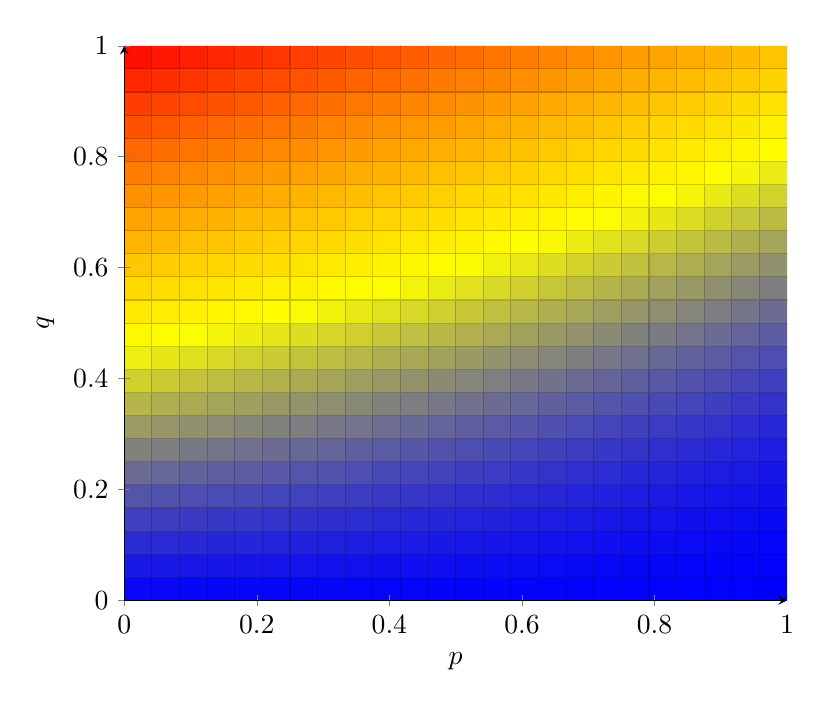
\begin{tikzpicture}
  \begin{axis}[
    view={0}{90},
    axis lines = left,
    xlabel = $p$,
    ylabel = $q$,
]]
    \addplot3[domain=0:1][surf] {(((x(1-y))/(x(2 - y) + y(1 - x) + y)) * x)+(((y(1-x))/(x (2 - y) + y(1 - x) + y)) * y)};
  \end{axis}
\end{tikzpicture}

% Probabilidade de o guarda chuva estar em casa

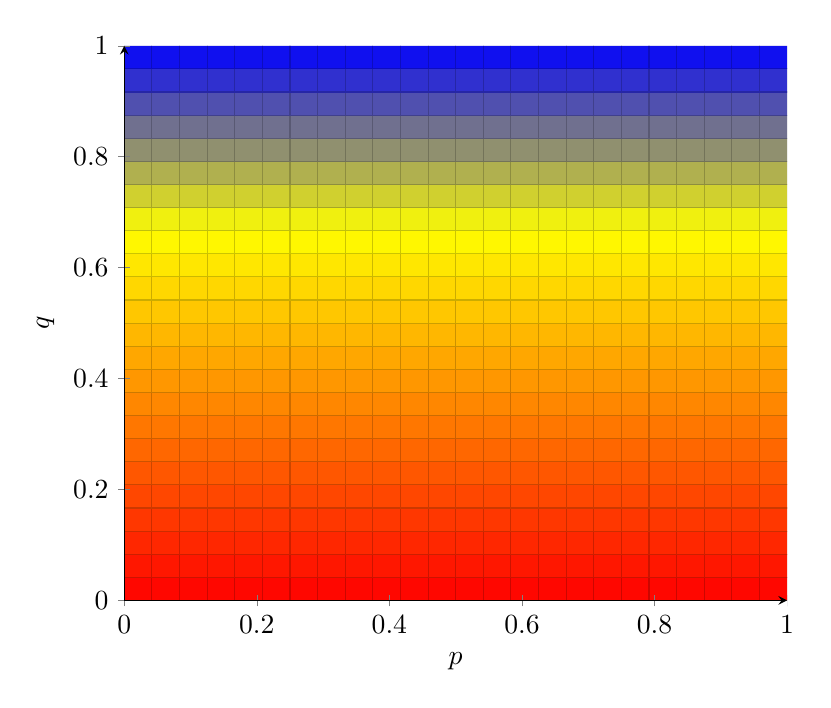
\begin{tikzpicture}
    \begin{axis}[
    view={0}{90},
    axis lines = left,
    xlabel = $p$,
    ylabel = $q$,
]]
    \addplot3[domain=0:1][surf] {( (x(y - 2))/(((2 * x)(y-1)) - (2 * y))};
  \end{axis}
\end{tikzpicture}



\end{document}
